\documentclass[12pt,a4paper]{article}

% Import basic packages first
\usepackage{tikz}
\usepackage{amsmath, amssymb}
\usepackage{geometry}
\usepackage{xcolor}
\usepackage{hyperref}
\usepackage[most]{tcolorbox}  % Added 'most' option
\usepackage{amsthm}

% Set page geometry
\geometry{margin=1in}

% Define colors
\definecolor{lightblue}{RGB}{173,216,230}
\definecolor{lightgreen}{RGB}{144,238,144}
\definecolor{pastelred}{RGB}{255,182,193}
\definecolor{pastelyellow}{RGB}{255,255,204}

% Define theorem-like environments
\theoremstyle{definition}
\newtheorem{definition}{Definition}[section]
\newtheorem{theorem}[definition]{Theorem}
\newtheorem{property}[definition]{Property}
\newtheorem{example}[definition]{Example}

% Custom box styles
\tcbset{
    theorembox/.style={
        colback=lightblue!10,
        colframe=lightblue!50,
        boxrule=0.5pt,
        left=2mm,
        right=2mm,
        top=1mm,
        bottom=1mm
    }
}

% Title information
\title{\Large\textbf{Graph Theory Visualization}\\[0.5em]
       \normalsize A Visual Guide to Graph Theory Concepts}
\author{\textbf{Your Name}\\
        Department of Mathematics}
\date{\today}

\begin{document}

% Title page
\maketitle

% Abstract or Introduction
\begin{tcolorbox}[theorembox]
\begin{abstract}
This document provides visual representations of fundamental graph theory concepts using TikZ. It includes examples of basic graphs, Euler paths, network flows, and spanning trees with detailed explanations and properties.
\end{abstract}
\end{tcolorbox}

\tableofcontents
\newpage

% First section with improved content
\section{Basic Graph Concepts}

\begin{definition}[Graph]
A graph G = (V, E) consists of a set V of vertices and a set E of edges, where each edge connects two vertices.
\end{definition}

\begin{property}[Degree]
The degree of a vertex is the number of edges incident to it.
\end{property}

\begin{center}
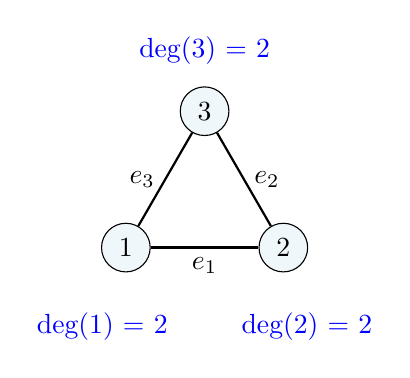
\begin{tikzpicture}
    % Create vertices with labels and degrees
    \node[draw, circle, fill=lightblue!20] (A) at (0,0) {1};
    \node[draw, circle, fill=lightblue!20] (B) at (2,0) {2};
    \node[draw, circle, fill=lightblue!20] (C) at (1,1.732) {3};
    
    % Draw edges with labels
    \draw[thick] (A) -- node[below] {$e_1$} (B);
    \draw[thick] (B) -- node[right] {$e_2$} (C);
    \draw[thick] (C) -- node[left] {$e_3$} (A);
    
    % Add degree annotations
    \node[text=blue] at (-0.3,-1) {deg(1) = 2};
    \node[text=blue] at (2.3,-1) {deg(2) = 2};
    \node[text=blue] at (1,2.5) {deg(3) = 2};
\end{tikzpicture}
\end{center}

\begin{theorem}[Handshaking Lemma]
The sum of degrees of all vertices in a graph is equal to twice the number of edges.
\end{theorem}

\section{Graph Properties}

\begin{tcolorbox}[theorembox]
Important properties of graphs include:
\begin{itemize}
    \item \textbf{Connectivity}: A graph is connected if there exists a path between any two vertices.
    \item \textbf{Planarity}: A graph is planar if it can be drawn without edge crossings.
    \item \textbf{Bipartiteness}: A graph is bipartite if its vertices can be divided into two disjoint sets.
\end{itemize}
\end{tcolorbox}

\begin{example}[Bipartite Graph]
\begin{center}
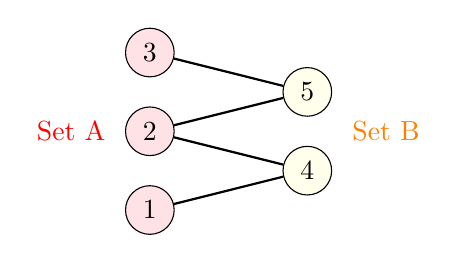
\begin{tikzpicture}
    % Left set vertices
    \node[draw, circle, fill=pastelred!40] (A1) at (0,0) {1};
    \node[draw, circle, fill=pastelred!40] (A2) at (0,1) {2};
    \node[draw, circle, fill=pastelred!40] (A3) at (0,2) {3};
    
    % Right set vertices
    \node[draw, circle, fill=pastelyellow!40] (B1) at (2,0.5) {4};
    \node[draw, circle, fill=pastelyellow!40] (B2) at (2,1.5) {5};
    
    % Draw edges
    \draw[thick] (A1) -- (B1);
    \draw[thick] (A2) -- (B1);
    \draw[thick] (A2) -- (B2);
    \draw[thick] (A3) -- (B2);
    
    % Add set labels
    \node[text=red] at (-1,1) {Set A};
    \node[text=orange] at (3,1) {Set B};
\end{tikzpicture}
\end{center}
\end{example}

\section{Graph Coloring}
\begin{tcolorbox}[theorembox]
A proper vertex coloring is an assignment of colors to vertices such that no adjacent vertices share the same color.
\end{tcolorbox}

\begin{center}
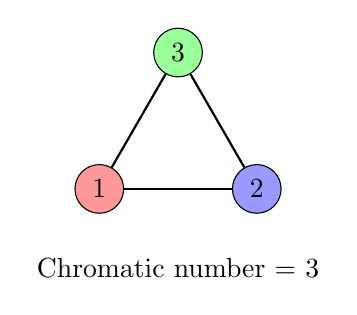
\begin{tikzpicture}
    % Create vertices with different colors
    \node[draw, circle, fill=red!40] (A) at (0,0) {1};
    \node[draw, circle, fill=blue!40] (B) at (2,0) {2};
    \node[draw, circle, fill=green!40] (C) at (1,1.732) {3};
    
    % Draw edges
    \draw[thick] (A) -- (B);
    \draw[thick] (B) -- (C);
    \draw[thick] (C) -- (A);
    
    % Add chromatic number
    \node[text=black] at (1,-1) {Chromatic number = 3};
\end{tikzpicture}
\end{center}

\begin{property}[Chromatic Number]
The chromatic number of a graph is the minimum number of colors needed for a proper vertex coloring.
\end{property}

\end{document}
